
\begin{figure*}[h!]%
 \centering
 \subfloat[Selecting a rotation angle manually]{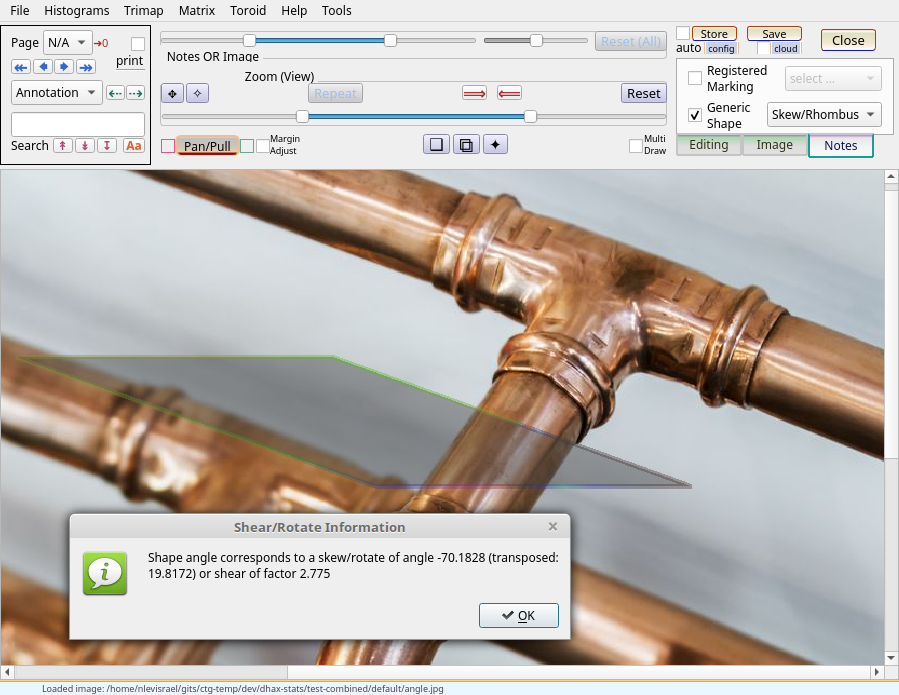
\includegraphics[width=0.93\textwidth, trim=0mm 0mm 0mm 80mm, clip]{images/set-angle.png}\label{fig:HOUGH-a}}\\
 \subfloat[GUI support for stepping through 
the evaluation transforms]{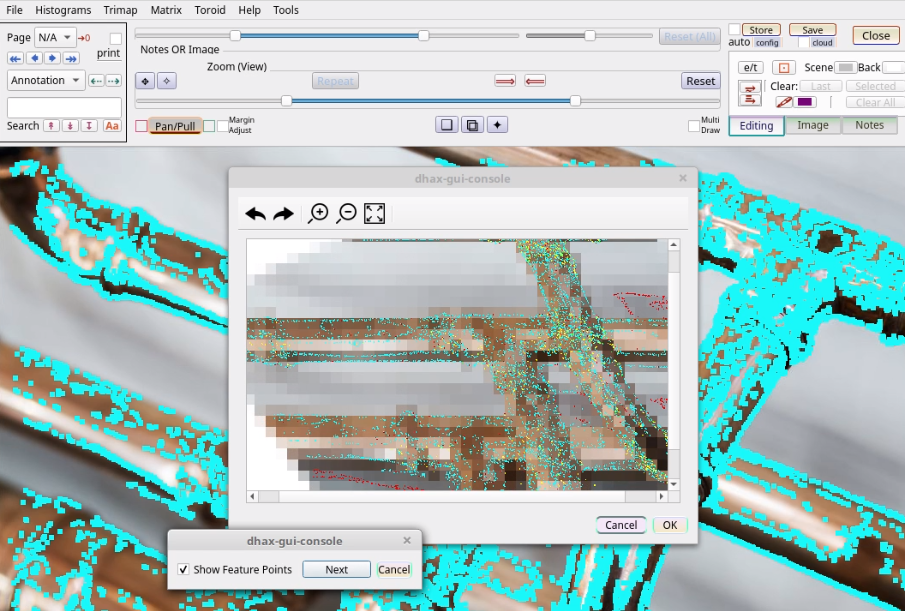
\includegraphics[width=\textwidth/2]{images/gui.png}\label{fig:HOUGH-b}}\hspace*{1em}
 \subfloat[Deriving a rotation angle via HOUGH line-detection]{\raisebox{3pt}{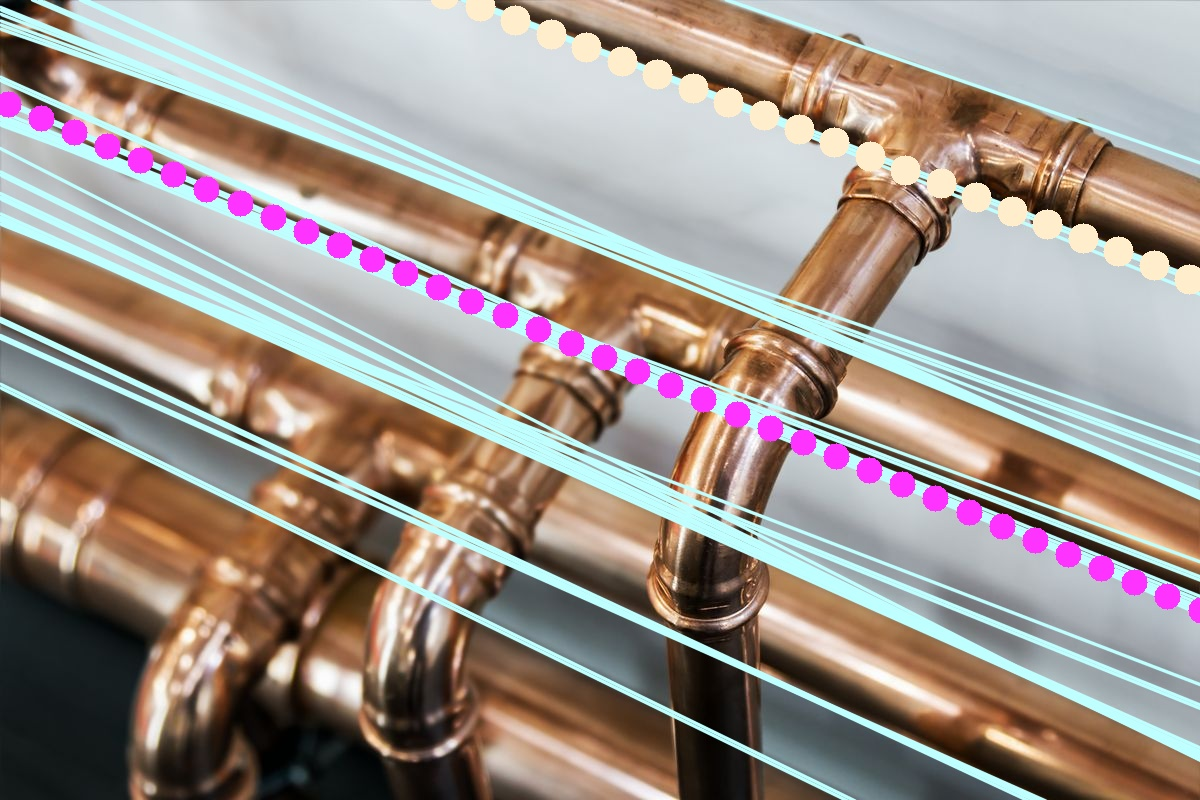
\includegraphics[width=.49\textwidth]{images/HOUGH.jpg}}\label{fig:HOUGH-c}}\\
 \subfloat[Evaluating how the keypoints map to binned 
foreground/background areas]{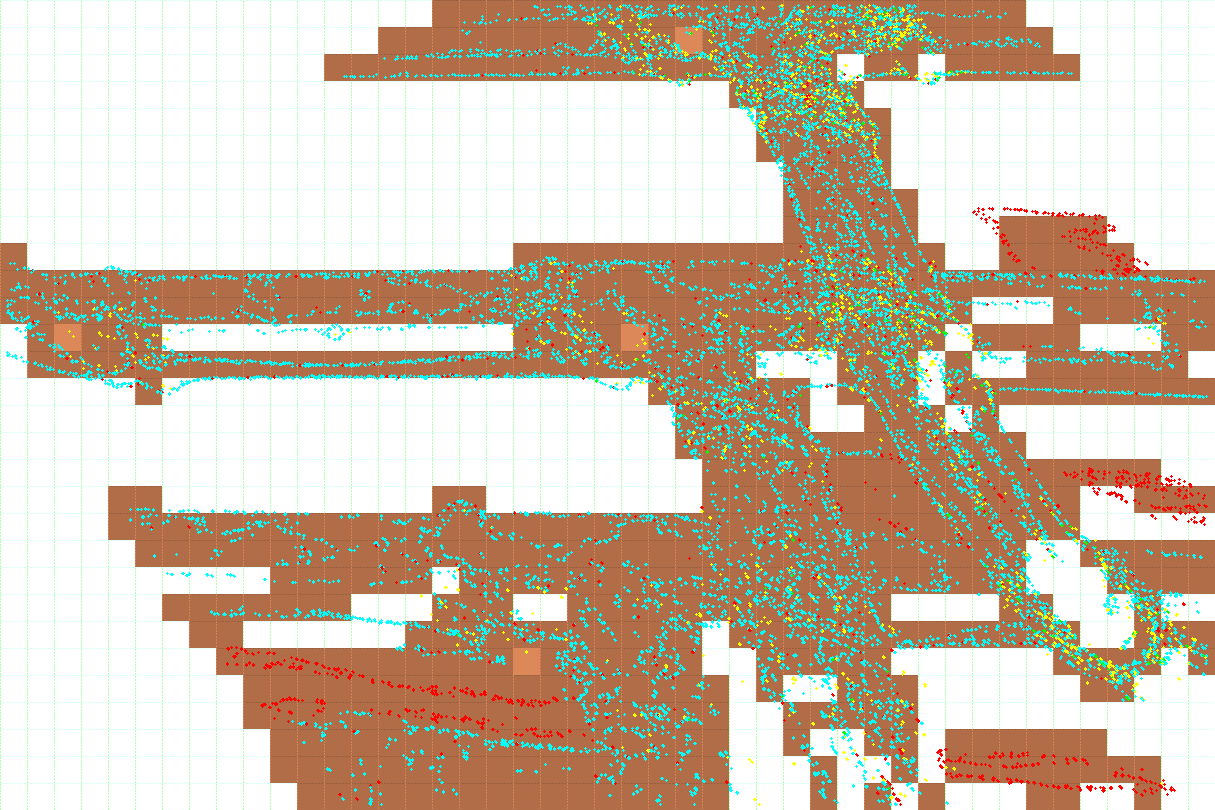
\includegraphics[width=\textwidth/2]{images/test.png}\label{fig:HOUGH-d}}\hspace*{2em}%
 \subfloat[The same HOUGH line detector run against a 
conventional grayscale reduction (average 
angles are magenta, target angle tan-orange)]{\raisebox{1em}{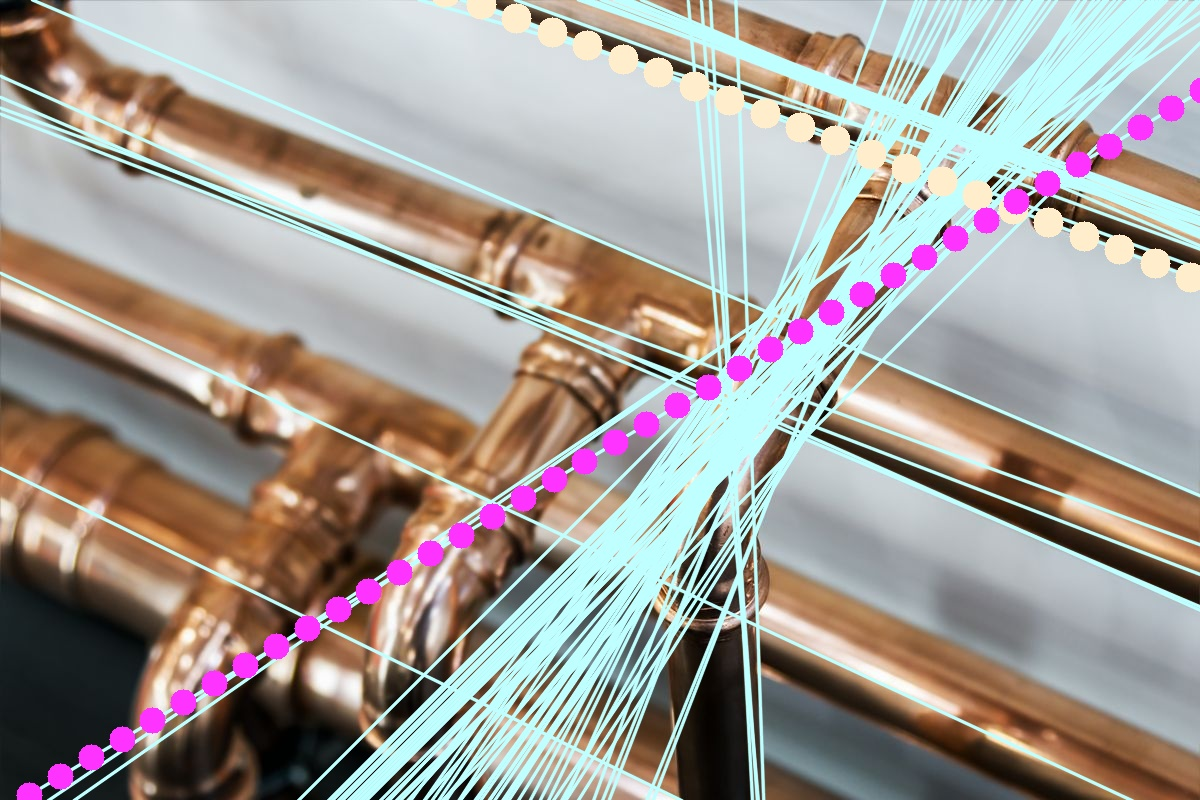
\includegraphics[width=.48\textwidth]{images/gray-HOUGH.jpg}}\label{fig:HOUGH-e}}\\
 \caption{Deriving a Rotation Angle for Evaluating the Keypoint Detector}%
 \label{fig:HOUGH-all}%
{\labelbox{To calculate how well the keypoints match 
the foreground, we transform the original image to yield 
orthogonal boxes, where it is easy to calculate how 
many keypoints (if any) lie on each box.  Visually, 
note that an automated HOUGH line-detector 
operating on an XCSD toroidal color space yields 
results comparable to manually selecting a global 
angular orientation for the image [a], [c].  Mapping 
the image to a skew/rotated and discretized box-set to 
quantify how closely the keypoints map to the foreground [b], [d].
Watershed methods (based on color-average inside each box, and 
their distance to the highest-probability foreground 
color) classify each box as approximating a foreground 
or background region.  For comparison, [e] shows a 
duplicate of [c]'s line-detector only using a 
conventional (realistic) grayscale conversion in 
lieu of XCSD channel-reduction; the latter analysis 
shows an entirely different (and mutually inconsistent) 
set of HOUGH lines.}}
\end{figure*}


